\section{Motivation: Coding Structure Can Guide KV}
\label{sec:motivation}

SWE-bench asks a model to resolve a GitHub issue against a real
repository~\cite{swebench}. Multi-agent wrappers split planner,
implementer, tester, and reviewer roles~\cite{multiagent2025,llmagents2024}.
Each role re-reads files that an earlier role already encoded, often
after a tool observation that shifts later tokens.
Figure~\ref{fig:dag-example} is that role graph. Trajectories come from
a 24-task Verified live-agent run (rolling-6 history, 28K prompt cap).
They are the evaluation substrate, not official Accuracy.

\begin{figure}[ht]
\centering
\resizebox{\columnwidth}{!}{\begingroup
\definecolor{ikvblue}{HTML}{2F6DB3}
\definecolor{ikvnavy}{HTML}{1B4F8A}
\definecolor{ikvteal}{HTML}{5BB3A7}
\definecolor{ikvorange}{HTML}{D96B2B}
\definecolor{ikvgray}{HTML}{6B6B6B}
\definecolor{rolep}{HTML}{D6E6F5}
\definecolor{rolec}{HTML}{D8F0EA}
\definecolor{rolet}{HTML}{FBE3D5}
\definecolor{roler}{HTML}{E8DEF4}
\begin{tikzpicture}[
  font=\sffamily\scriptsize,
  >=Stealth,
  role/.style={rounded corners=2pt, align=center,
    minimum width=2.05cm, minimum height=0.72cm, inner sep=3pt},
]
\node[role, draw=ikvblue, fill=rolep] (p) {Planner};
\node[role, draw=ikvteal, fill=rolec, right=0.85cm of p] (c) {Implementer};
\node[role, draw=ikvorange, fill=rolet, right=0.85cm of c] (t) {Tester};
\node[role, draw=ikvnavy, fill=roler, right=0.85cm of t] (r) {Reviewer};
\draw[->, ikvgray] (p) -- (c);
\draw[->, ikvgray] (c) -- (t);
\draw[->, ikvgray] (t) -- (r);

\node[draw=ikvblue, fill=white, rounded corners=2pt, inner sep=3pt,
  text width=8.6cm, align=left, below=0.55cm of c] (file) {%
  Same \texttt{repository\_code} file, e.g.\ \texttt{mod.py}\\
  later role rereads it at a shifted index ($\Delta \neq 0$)};

\draw[->, ikvblue] (p.south) -- ++(0,-0.18) -| ($(file.north)+(-2.6,0)$);
\draw[->, ikvteal] (c.south) -- ++(0,-0.18) -| ($(file.north)+(-0.7,0)$);
\draw[->, ikvorange] (t.south) -- ++(0,-0.18) -| ($(file.north)+(0.7,0)$);
\draw[->, ikvnavy] (r.south) -- ++(0,-0.18) -| ($(file.north)+(2.6,0)$);

\node[font=\sffamily\scriptsize, text=ikvgray, above=0.12cm of c] {rolling-6 coding protocol};
\end{tikzpicture}
\endgroup
}
\caption{Coding roles reread the same file module at a shifted index.}
\Description{Planner, implementer, tester, and reviewer reread the same file module.}
\label{fig:dag-example}
\end{figure}

\subsection{Complementary reuse the prefix cache cannot take}

Figure~\ref{fig:motivation-coverage} (top) measures the split on the 7B
PLAN (job 137185 tokens, no new GPU). Every group has a nonempty radix
LCP \emph{and} a shifted file island. Mean LCP is $24.7\%$ of the
target prompt ($1047$ tok.); file-module copy is $33.4\%$ ($1537$ tok.).
The two token sets are disjoint (zero overlap, and LCP never reaches
the first island). Prefix caches and CacheWise can take the left
$24.7\%$; they cannot map the shifted $33.4\%$.

Unconstrained shifted copy does not stop at those file islands.
Figure~\ref{fig:motivation-extra} (bottom) compares the 7B file-module
PLAN with the KVCOMM-style PLAN from job 137400 (same target ids, no
new GPU). The clone copies a campaign total of $194{,}624$ extra tokens
in $235/235$ groups (spans the file gate refused). Almost every
file-module token sits inside an unconstrained span ($360{,}734$
shared; $425$ file-only). A general copier is faster because it moves
those bytes; they are matching context, not version-valid repository
files.

\begin{figure}[ht]
\centering
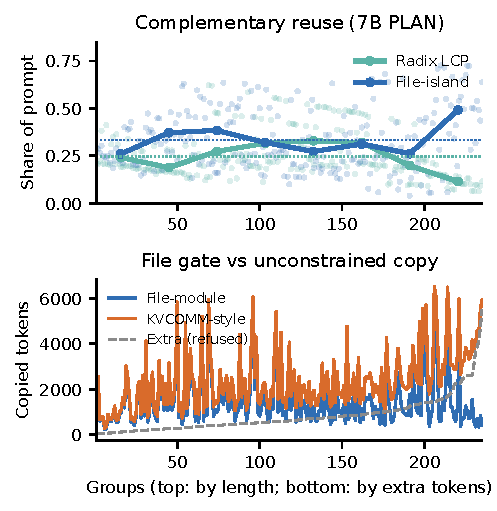
\includegraphics[width=\columnwidth]{figures/fig_motivation_coverage.pdf}
\caption{Top: complementary reuse on the 7B PLAN ($235$ groups). Mean
LCP $24.7\%$; file-island $33.4\%$; overlap $0$. Bottom: file-module
versus unconstrained copy (job 137400 PLANs). Extra $194{,}624$ tokens
in $235/235$ groups. Not a new GPU arm and not
Table~\ref{tab:eval-summary}.}
\Description{Line charts of LCP vs file-island share and of copied tokens vs unconstrained extra.}
\label{fig:motivation-coverage}
\label{fig:motivation-extra}
\end{figure}

\subsection{Where the loss sits}
\label{sec:attn-proxy}

The 7B speed campaign in Section~\ref{sec:evaluation} does not record
attention. A separate, frozen probe on Qwen2.5-Coder-3B~\cite{qwen25}
asks only where the activation error lives after a true-lossy file-island
splice. It is not 30B native attention, not official resolved, and not
the admit rule: the compiler in Section~\ref{sec:template} still uses
token-ID equality, not Attention scores.

Figure~\ref{fig:tv-locus} and Figure~\ref{fig:attn-proxy} report that
probe. TV here is the total-variation \emph{distance between two
attention distributions} (Dense versus splice), not a synonym for the
KV tensors. On 26 single-island targets (13 tasks) that median
attention TV is $0.00264$ on the recomputed suffix and $0.00492$ at
the next-action marker, but $0.0462$ on the copied island's
\emph{source-time formation} (about $4.4\%$ of that formation mass has
no counterpart in the target prefix). On 20 Dense
prompts the last 32 query tokens put median $80.1\%$ of attention on the
top $10\%$ of keys (within-observation top-$20\%$ mass $80.2\%$). An
eight-prompt same-input diagnostic puts coding-aware module TV at
$0.00214$ against $0.0454$ (CacheBlend) and $0.0745$ (KVCOMM); that
comparison is local TV, not matched-coverage Accuracy
(Figure~\ref{fig:module-tv}).

\begin{figure}[ht]
\centering
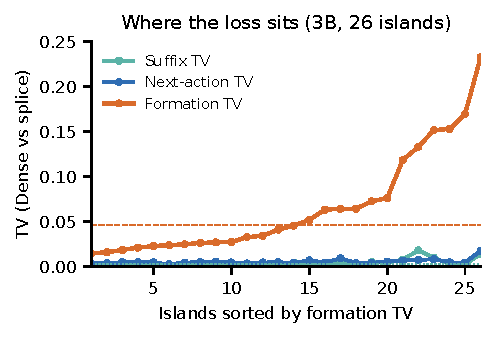
\includegraphics[width=\columnwidth]{figures/fig_tv_locus.pdf}
\caption{Per-island attention total-variation (TV) after a file-island
splice (Qwen2.5-Coder-3B, $26$ islands, sorted by formation TV).
TV is attention-distribution distance, not a KV-cache quantity.
Suffix attention does not collapse; formation TV is an order of
magnitude larger (frozen medians $0.00264$ / $0.00492$ / $0.0462$).
Not 30B native and not Table~\ref{tab:eval-summary}.}
\Description{Line chart of suffix, next-action, and formation TV across 26 islands.}
\label{fig:tv-locus}
\end{figure}

\begin{figure}[ht]
\centering
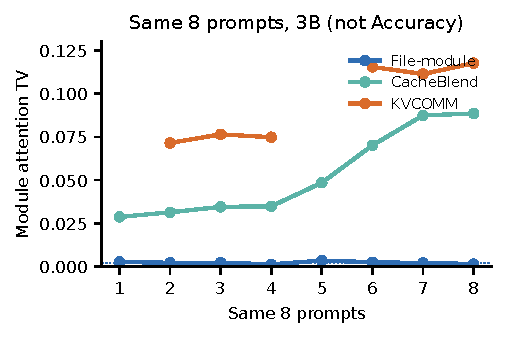
\includegraphics[width=\columnwidth]{figures/fig_module_tv.pdf}
\caption{Same eight prompts, 3B: per-prompt module attention TV of
file-module copy versus CacheBlend and KVCOMM. Local TV, not Accuracy
and not 7B TTFT.}
\Description{Line chart of module attention TV for three methods on eight prompts.}
\label{fig:module-tv}
\end{figure}

\begin{figure}[ht]
\centering
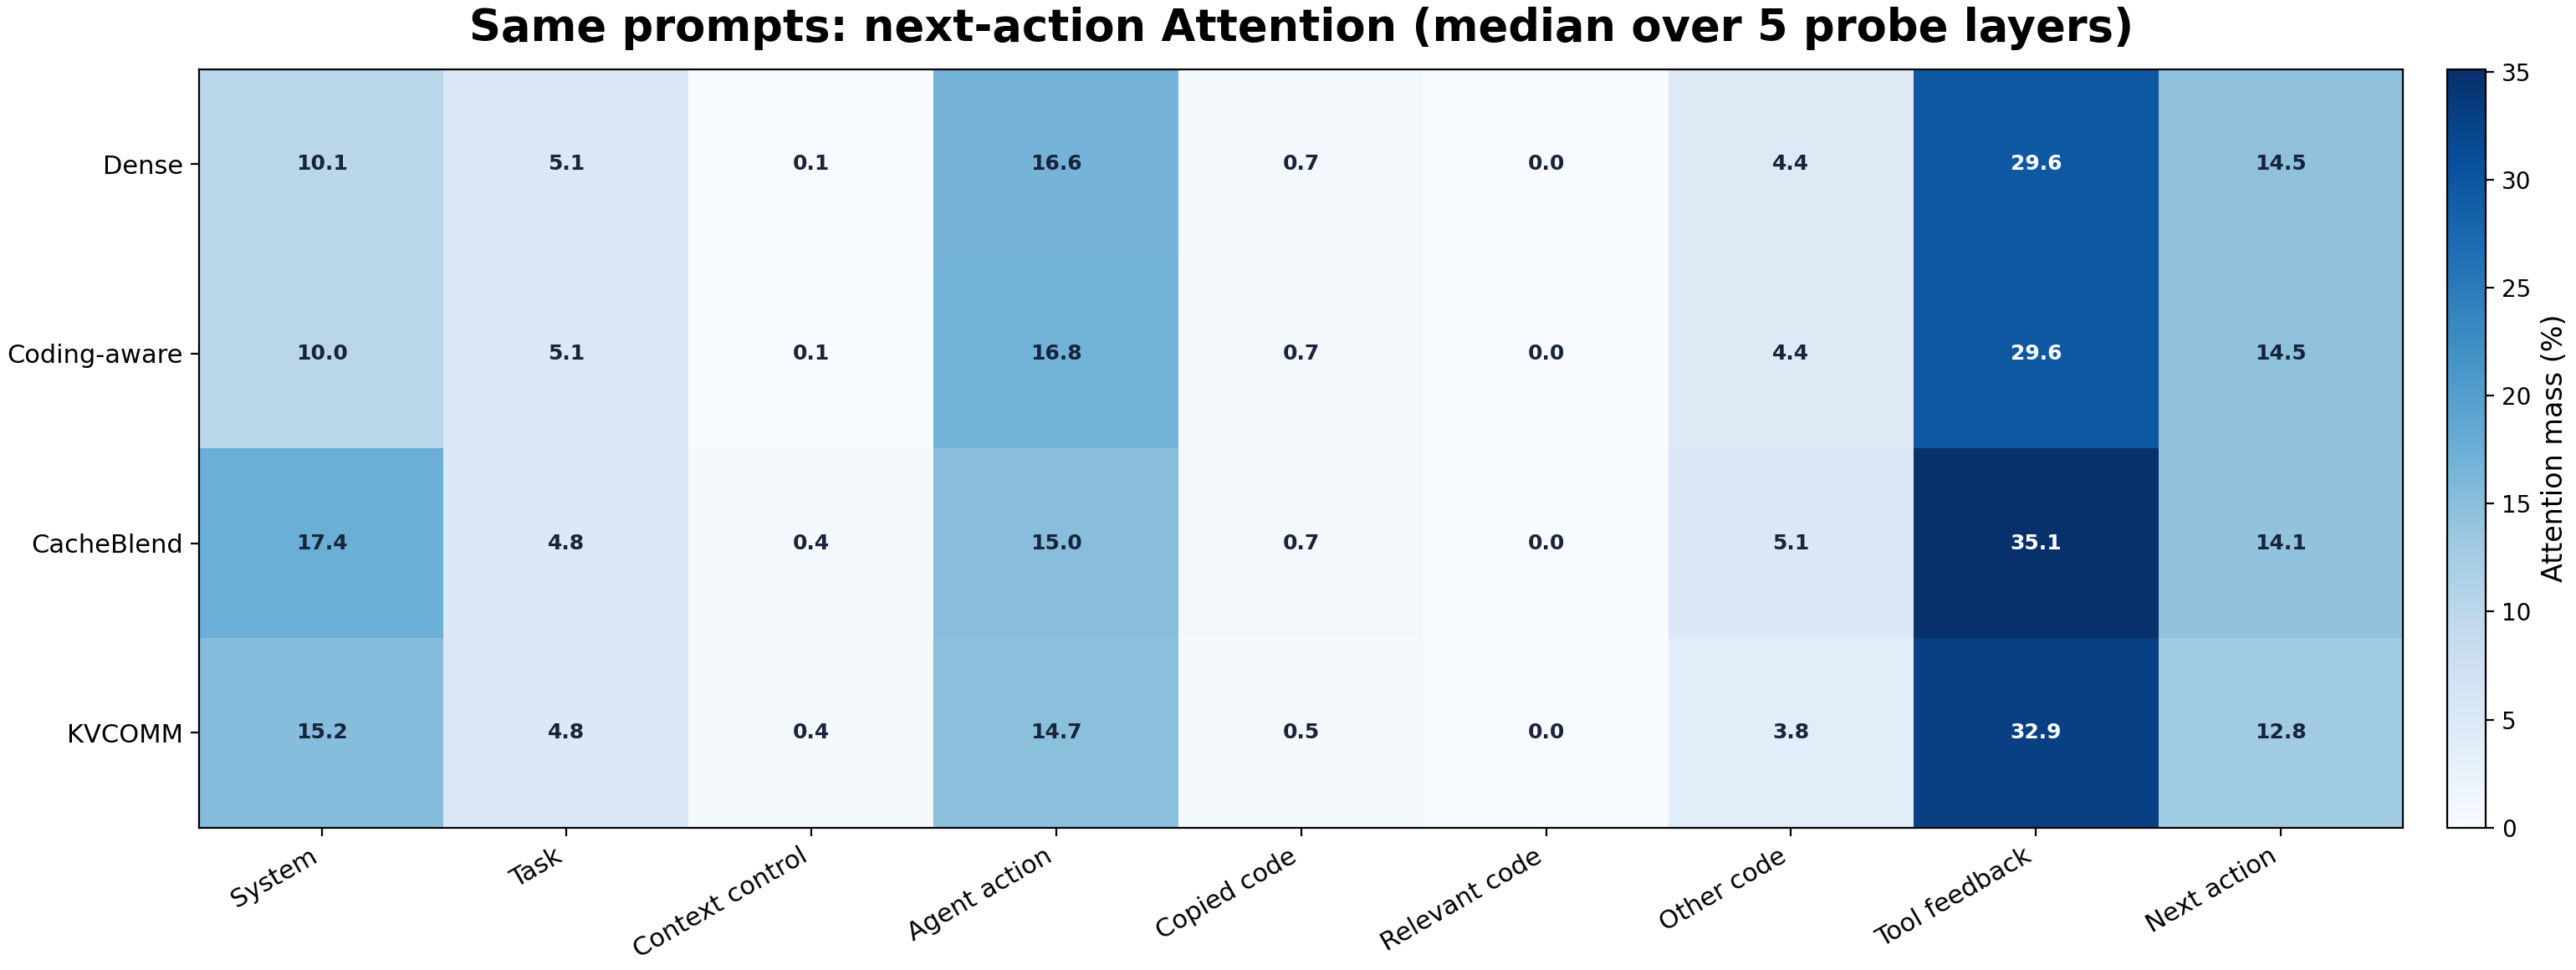
\includegraphics[width=\columnwidth]{figures/fig_attn_heatmap.png}
\caption{Next-action attention mass by prompt region, median over probe
layers (same eight 3B prompts). File-module copy tracks Dense; CacheBlend
and KVCOMM overweight system and tool-feedback tokens. Not
Table~\ref{tab:eval-summary}.}
\Description{Heatmap of attention mass by method and region.}
\label{fig:attn-heatmap}
\end{figure}

\begin{figure}[ht]
\centering
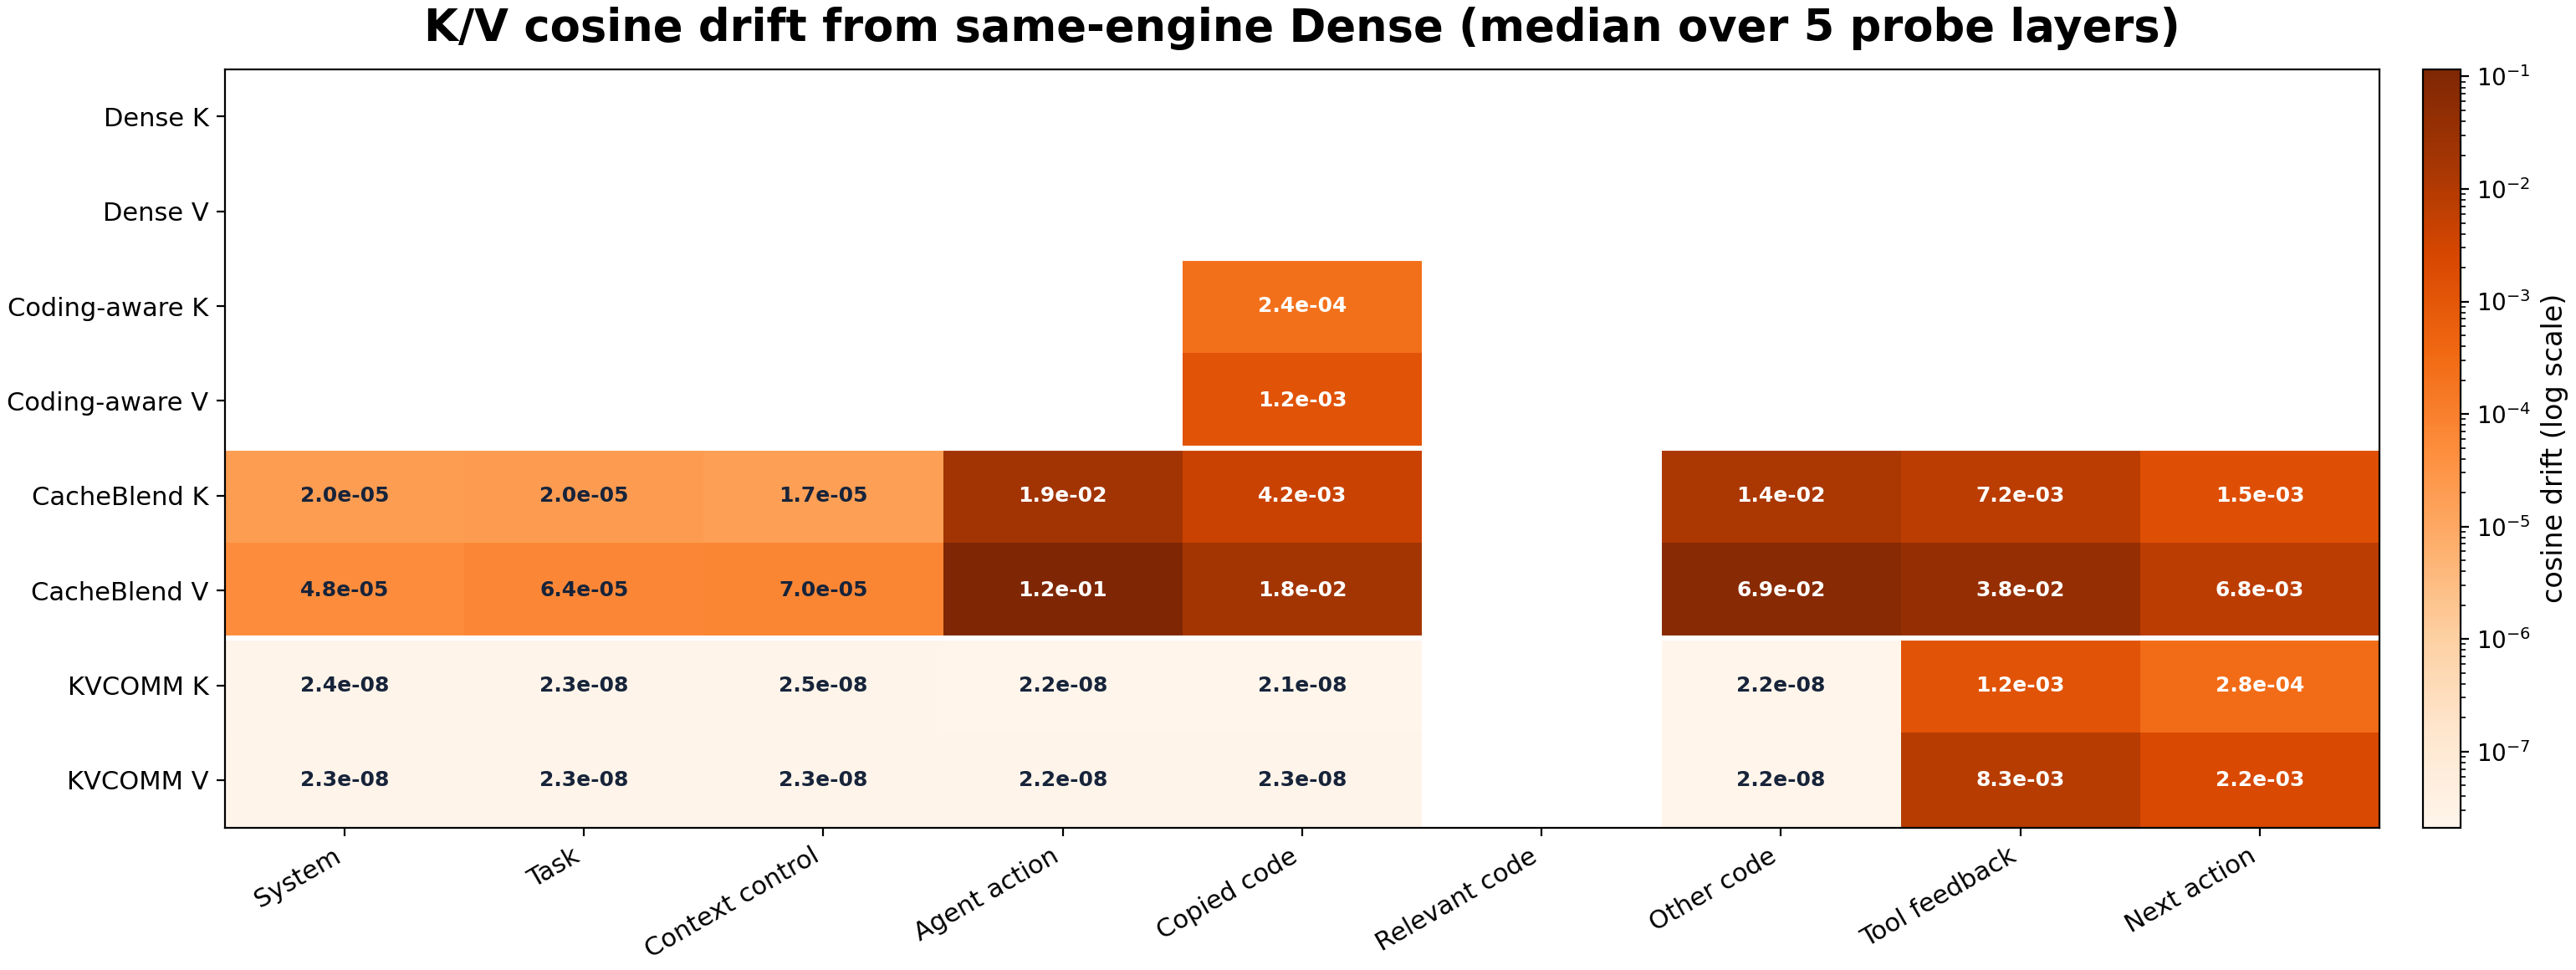
\includegraphics[width=\columnwidth]{figures/fig_kv_heatmap.png}
\caption{$K/V$ cosine drift from same-engine Dense (same eight 3B
prompts). File-module drift is confined to the copied code island;
CacheBlend and KVCOMM drift on agent-action, other-code, and tool
spans. Not 7B TTFT.}
\Description{Heatmap of KV cosine drift by method and region.}
\label{fig:kv-heatmap}
\end{figure}

\begin{figure}[ht]
\centering
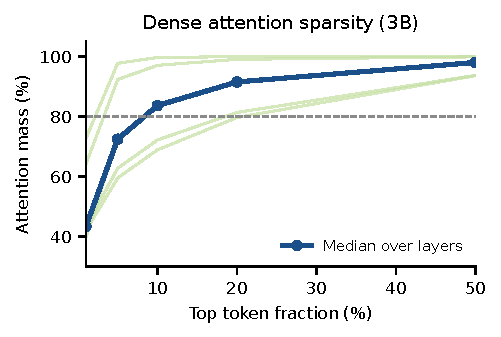
\includegraphics[width=\columnwidth]{figures/fig_attn_proxy.pdf}
\caption{Frozen 3B Dense sparsity, not the 30B TTFT campaign. Median
top-$10\%$ key mass $80.1\%$ ($n{=}20$); within-observation top-$20\%$
mass $80.2\%$. Not official resolved.}
\Description{Line chart of cumulative attention mass versus top token fraction.}
\label{fig:attn-proxy}
\end{figure}

The implication is directional, not a quality ranking: suffix attention
does not collapse after a file-module copy, so a suffix-recompute copier
is the wrong default repair. The larger drift is how the island's $K/V$
formed under the source prefix. Unconstrained copiers additionally drift
on tool and agent spans the file gate refused.

\subsection{Opportunities}
\label{sec:opportunities}

Three opportunities follow, and they are the design of
Section~\ref{sec:problem}.

\begin{enumerate}[leftmargin=1.2em,itemsep=0.12em]
    \item \textbf{Admit the shifted file, not the whole prompt.}
          $33.4\%$ of the target is a version-valid
          \texttt{repository\_code} island at $\Delta\neq 0$, disjoint
          from the $24.7\%$ radix prefix. A coding-aware engine can copy
          that island and leave issue text, tool logs, and stale files
          Dense.
    \item \textbf{Correct $K$ phase; do not recompute the suffix.}
          Formation TV is ${\sim}17\times$ suffix TV. Source-side $K$
          pre-rotation under the known $\Delta$, with $V$ copied as-is,
          matches where the residual actually lives.
    \item \textbf{Fail closed on a mechanically invalid island.}
          Token-hash mismatch, incomplete coverage, or allocation
          failure must discard the whole island rather than splice a
          partial page. Unconstrained copy of the extra $194{,}624$
          tokens is faster and less agreed; it is not the policy.
\end{enumerate}
